\section{Inledning}

\begin{figure}
	\centering
	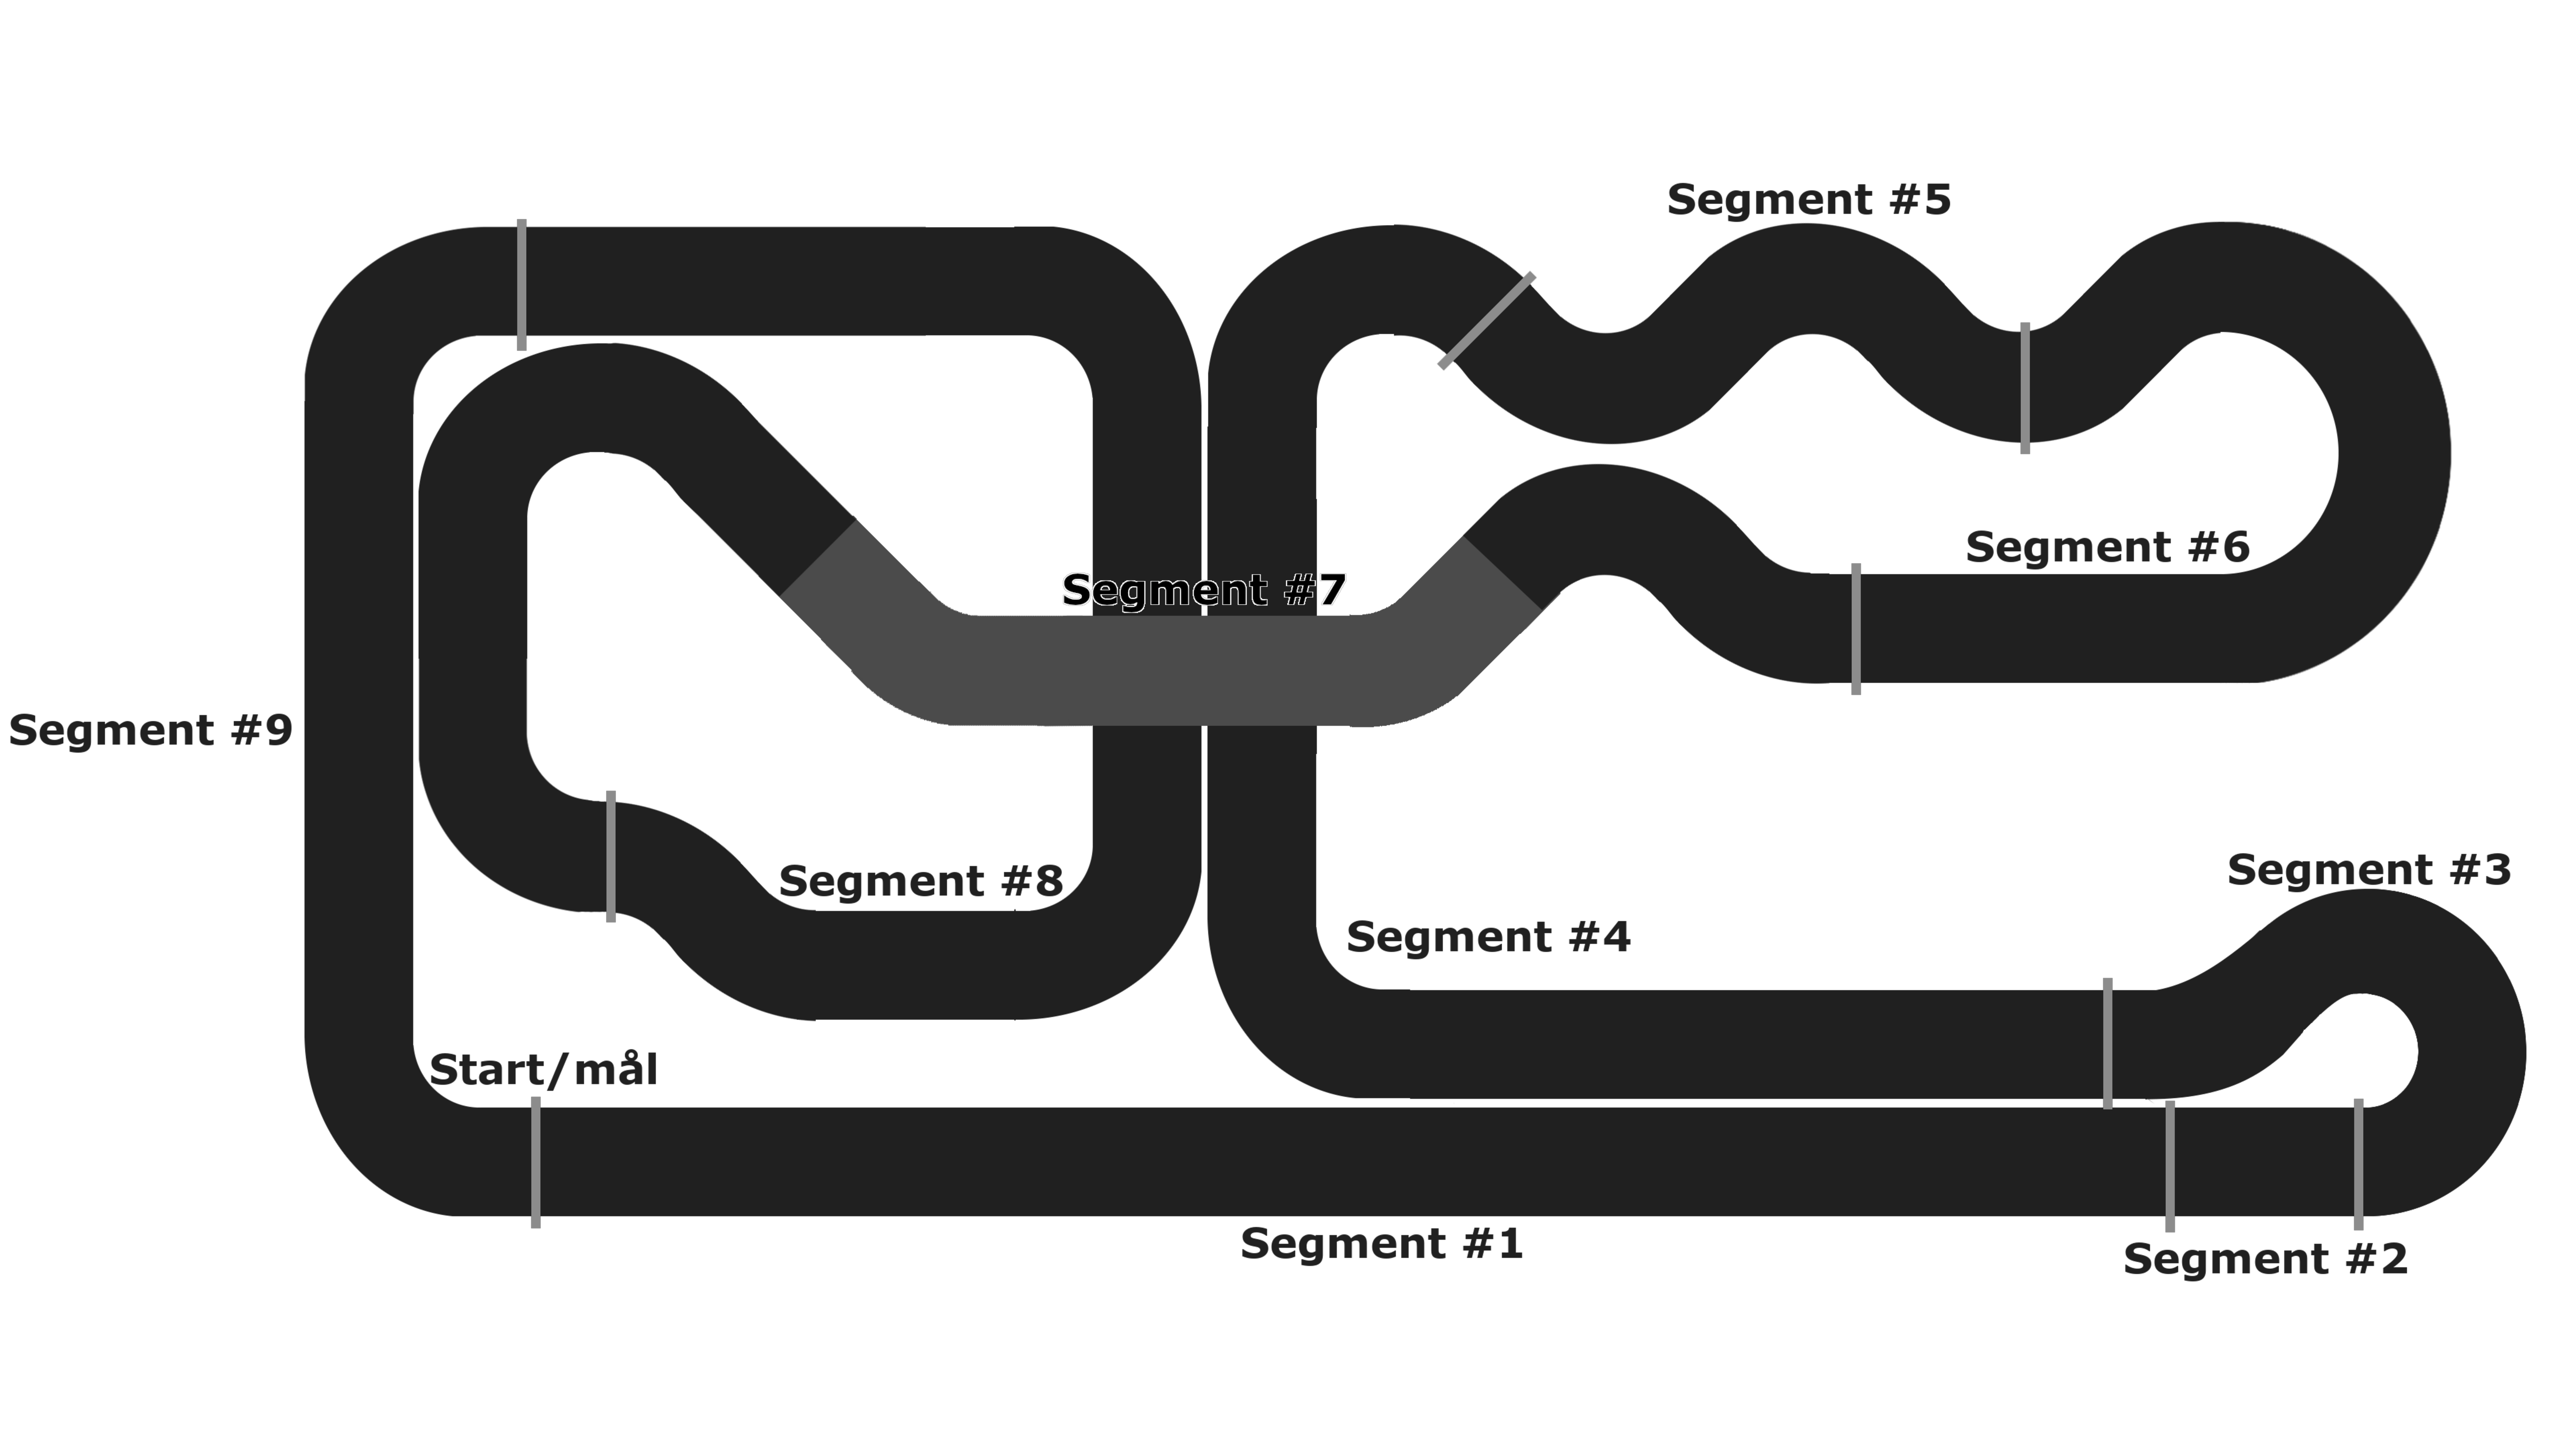
\includegraphics[width=\linewidth] {Figures/BanaModell}
	\caption{En modell av bilbanan.}
	\label{fig:bilbanan}
\end{figure}

\subsection{Bakgrund} Projektet har utförts med hjälp av en bilbana samt
flera bilar, givare, spänningsaggregat och två datorer inne i bilbanerummet. Via datorn har spänning tillförts till bilbanan. Med hjälp av givarna är
det möjligt att veta när en bil har passerat en givare.  Programvaran har utvecklats
i Matlab.

\subsection{Syfte och mål}

Syftet med projektet är att lära sig att arbeta i projekt utifrån
projektmodellen Lips. Målet med projektet är att konstruera ett system som bland
annat ska få bilarna att köra runt en bilbana på en vald referenstid mellan 12
och 15 sekunder. Detta ska uppfyllas för båda banor, för flera bilar med olika
egenskaper och med maximalt 5 kalibreringsvarv. Fler krav som ska klaras av
finns i kravspecifikationen. Se kravspecifikationen \ref{app:kravbeskrivning}
samt kursmål.

